\section{RAOES Overview}
\label{sec:overview}
The goal of RAOES is to seamlessly support the collaboration of software architects and programmers in developing event-driven systems.
In the latter, the behavior of active objects is specified by using UML State Machines.
As previously described, it is very difficult to reconstruct the original model from the generated code since there is no bijective mapping between these artifacts.
Therefore, RAOES defines a textual interface embedded inside the active objects, which are defined by object-oriented classes. 
This mechanism acts as a role to communicate the C++ programming language to USM so that the traceability between model and code in the reverse direction of the RTE can be eased.

\begin{figure}
	\centering
	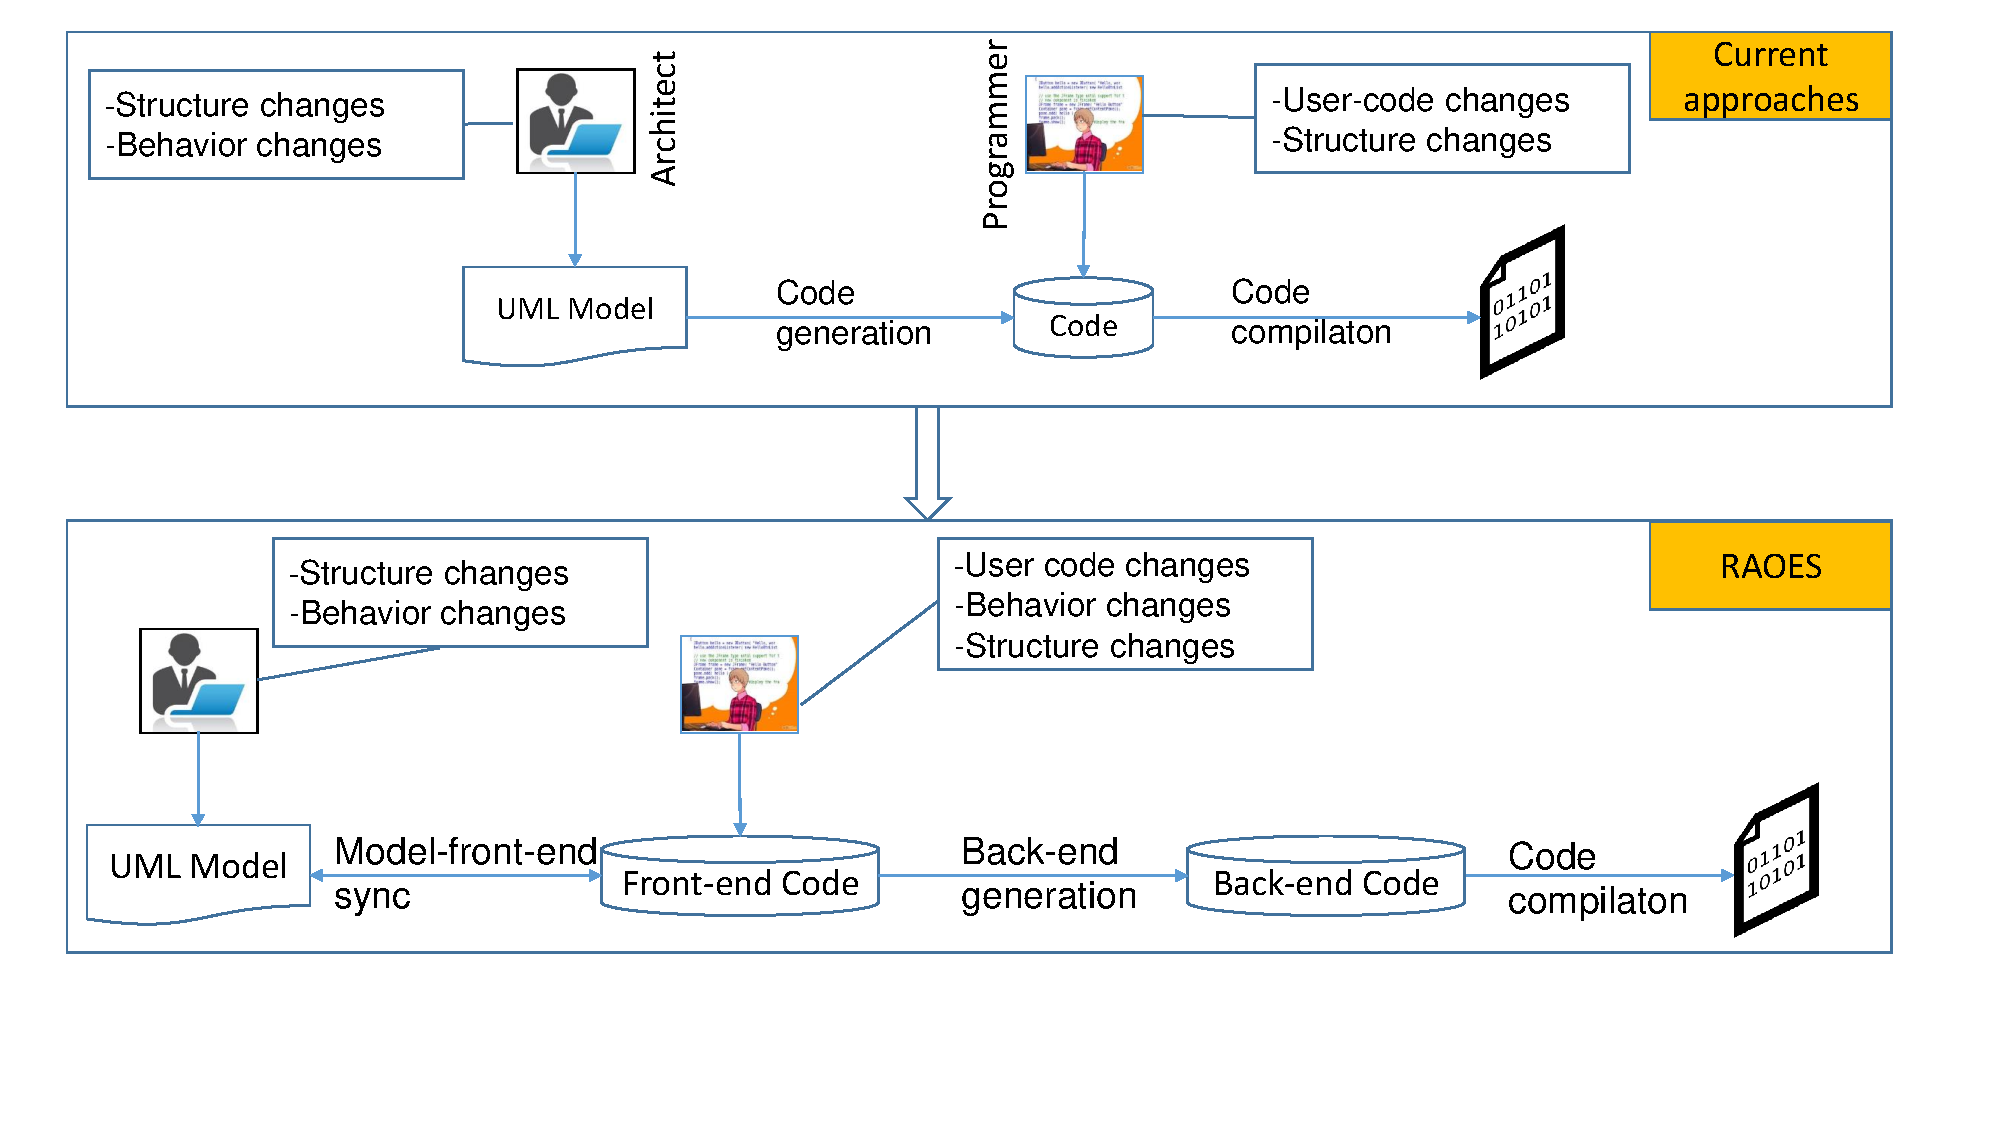
\includegraphics[clip, trim=0.6cm 6.4cm 1.4cm 0.5cm, width=1.0\columnwidth]{figures/frontend}
	\caption{From existing approaches to RAOES} 
	\label{fig:raoes}
\end{figure}

Specifically, in the code generation process, instead of directly generating C++ code as in Listing \ref{lst:generated1}, RAOES produces a front-end C++ code.
The latter is an intermediate representation, which is C++-conformant.
Fig. \ref{fig:raoes} shows how RAOES is different from the existing code generation approaches.
RAOES separates codes for the structural and behavioral part.
The connections between these parts are realized by using simple name binding mechanisms.

For example, by using RAOES, the generated front-end code for the example in Fig. \ref{fig:illustration} (a) is presented in Listing \ref{lst:front-end1}.
The USM defining the behavior of the active class \ti{System} is defined inside the class.
The USM is written in a description-like language.
The topology of the USM is explicitly and hierarchically described.
All USM features can be represented in RAOES's front-end.
Hence, we allow to fully generate code from USMs.

\lstinputlisting[language=C++, caption=Front-end code generated from the USM example in Fig. \ref{fig:illustration} (a), label=lst:front-end1,frame=f]{code/front-end1.cpp}

In RAOES, the programmers can modify not only structural and user-code parts, which are offered by advanced round-trip engineering tools such as Rhapsody and Enterprise Architect, but also the high-level logic behavior specified by USM.
The modification is realized by making changes to the front-end code.
For the evolution of the state \ttt{S2} from the USM in \ref{fig:illustration} (a) to that of Fig. \ref{fig:illustration} (b), the programmers must do some steps: (1) delete the three vertexes \ttt{Enp1}, \ttt{h1}, and final state of \ttt{S2} by deleting the lines 6, 7, and 9 in Listing \ref{lst:front-end1}, and the transition \ttt{t5} (not shown in Listing \ref{lst:front-end1}); and 
(2) add the deep history \ttt{dh1} (line 2 in Listing \ref{lst:front-end2}), and update the transitions as the lines 12-13 in Listing \ref{lst:front-end2}.
If the programmers wish to modify the low level behavior, they can simply modify user-code as usual C++ method code, for example the method \ttt{S11\_entry} in Listing \ref{lst:front-end1}.
Other parts such as user-created attributes or methods can be freely modified.






\lstinputlisting[language=C++, caption=Front-end code generated from the USM example in Fig. \ref{fig:illustration} (b), label=lst:front-end2,frame=f]{code/front-end2.cpp}


The front-end closely connects to the USM concepts to enable programmers to modify the state machine.
The front-end integrates and merges the USM description into the active class \ti{System} and keeps the class members intact. 
Therefore, the programmers are free to work with C++ as their practice.
This is a particular difference of our approach and an advantage over some text-based state machine languages such as Umple \cite{lethbridge2010umplification} and ThingML \cite{thingml}.
The latter languages adapt existing languages and the programmers' habit into USMs by providing a new language with a new editor (usually defined in Eclipse Xtext).
However, the new editor usually does not support the IDE utilities such as syntax highlights and intelligent completion for mainstream programming languages. 



